%! TEX program = xelatex

\PassOptionsToPackage{quiet}{xeCJK}
\documentclass[withoutpreface,bwprint]{cumcmthesis}
\usepackage{etoolbox}
\usepackage{ctex}
\BeforeBeginEnvironment{tabular}{\zihao{-5}}
% 参考文献改用纯tex格式，不再需要natbib+bibtex
\usepackage[framemethod=TikZ]{mdframed}
\usepackage{url}
\usepackage{array}
\usepackage{tabularx}
\usepackage{longtable}
\newcolumntype{C}{>{\centering\arraybackslash}X}
\newcolumntype{R}{>{\raggedleft\arraybackslash}X}
\newcolumntype{L}{>{\raggedright\arraybackslash}X}

\usepackage{tikz}
\usetikzlibrary{arrows.meta}
\tikzset{
  box/.style={rectangle, draw, minimum width=3.2cm, minimum height=0.9cm, align=center},
  arrow/.style={thick, -{Stealth}}
}

\title{蔬菜类商品的自动定价与补货决策}

%%%%%%%%%%%%%%%%%%%%%%%%%%%%%%%%%%%%%%%%%%%%%%%%%%%%%%%%%%%%%
%% 正文
\begin{document}

% 标题
{\centering\zihao{3}\bfseries 蔬菜类商品的自动定价与补货决策\par}

\setcounter{page}{1}

\thispagestyle{empty}


\begin{abstract}

蔬菜类商品保鲜期短、品相随时间变差，商超需每日做出补货与定价决策。本文基于某商超2020年7月至2023年6月六个蔬菜品类251个单品的销售流水、批发价格和损耗率数据，建立了从品类关联分析、品类级补货定价到单品级选品优化的递进式数学模型。

\textbf{对于问题一,} 首先对销售流水按品类和日期聚合，经正态性检验发现全部品类拒绝正态分布假设，采用Spearman秩相关系数分析品类间关联关系，接着使用K-means++聚类算法对159个销售稳定的单品按销量规模和波动性聚类，最后对各品类日销售量进行分布拟合。结果表明，Spearman $\rho$ 范围为$[-0.194, 0.625]$，花叶类与花菜类关联最强（$\rho=0.625$），单品被聚为低量高波动与高量中波动两类（Silhouette=0.463），对数正态分布最能刻画蔬菜日销售量的分布形态。

\textbf{对于问题二,} 首先建立Prophet时间序列分解模型分离趋势、周/年季节性和中国节假日效应，接着从数据自行估计各品类需求价格弹性，然后建立约束报童模型以加成率和订货量为联合决策变量，通过二维网格搜索求解最优补货与定价策略。结果表明，单日总期望利润为2,918元（折扣回收率$k=0.66$，$k\in[0.50,0.75]$对应区间$[2,362,\;3,713]$元），较ARIMA+固定加成baseline（723元/天）提升304\%。优化加成率在103.6\%--128.2\%之间，品类间有充分区分。

\textbf{对于问题三,} 首先从6月24--30日可售品种中过滤日均销量$\geq 2.5$ kg的单品得到31个（恰好落在27--33范围内），接着各单品独立运行报童优化确定订货量与定价。结果表明，单日总期望利润为1,327元，较固定加成baseline（465元）提升185\%。全部六个品类需求满足率均超过78\%，水生根茎类最低（78.6\%），其余品类超过150\%。

\textbf{对于问题四,} 基于前三问建模过程中实际暴露的数据局限性，建议商超优先采集每日库存与缺货记录、折扣原因分类码和天气数据，以提高最敏感参数$k$的估计精度和需求预测质量。模型具有清晰的数学结构和可解释的参数，关键数值结论均经过参数扰动和敏感性检验。

\keywords{蔬菜定价；补货决策；Spearman秩相关；Prophet时间序列分解；报童模型；K-means++聚类}

\end{abstract}

\thispagestyle{empty}

\tableofcontents
\thispagestyle{empty}
\newpage

\setcounter{page}{1}


\section{引言}
\subsection{问题背景}

生鲜商超中蔬菜类商品保鲜期短，品相随销售时间增加而变差，大部分品种当日未售出则隔日无法再售。商超需根据历史销售和需求情况每日补货，但进货交易时间在凌晨3:00--4:00，商家须在不确切知道具体单品和进货价格的情况下做出补货决策。蔬菜的定价一般采用成本加成定价方法，商超对运损和品相变差的商品通常进行打折销售。可靠的市场需求分析对补货决策和定价决策尤为重要。从需求侧看，蔬菜类商品销售量与时间存在关联关系；从供给侧看，蔬菜供应品种在4月至10月较为丰富，商超销售空间的限制使得合理的销售组合极为重要。

题目提供某商超六个蔬菜品类（花叶类、辣椒类、食用菌、水生根茎类、茄类、花菜类）共251个单品的数据：附件1为商品信息，附件2为2020年7月1日至2023年6月30日的销售流水明细（878,503条交易记录），附件3为同期批发价格数据，附件4为近期损耗率数据。本文仅使用附件4中的可见工作表（单品级损耗率），品类级损耗率通过附件1与附件4的关联自行计算。

\subsection{问题重述}

\textbf{问题1：} 分析蔬菜各品类及单品销售量的分布规律及相互关系。

\textbf{问题2：} 以品类为单位，分析销售总量与成本加成定价的关系，给出各品类2023年7月1--7日的日补货总量和定价策略，使商超收益最大。

\textbf{问题3：} 在销售空间有限的情况下制定单品补货计划，可售单品总数27--33个，各单品订购量$\geq 2.5$ kg。根据6月24--30日可售品种，给出7月1日的单品补货量和定价策略，在尽量满足市场对各品类需求的前提下使收益最大。

\textbf{问题4：} 建议商超还需采集哪些数据，说明这些数据对解决上述问题的帮助和理由。



\section{总体分析}

本文的四个问题构成从描述性分析到优化决策再到建议的递进逻辑链条。问题一通过对历史销售数据进行统计分析和聚类，揭示蔬菜品类及单品的销售分布规律和关联关系，为后续建模提供特征选择依据。问题二在问题一的基础上，以品类为单位建立需求预测与报童优化模型，确定品类级的最优补货量和定价策略。问题三进一步细化到单品层面，在销售空间约束下筛选单品并逐一优化，使品类需求得到充分满足。问题四基于前三问建模过程中实际暴露的数据局限性，提出有针对性的数据采集建议。四个问题环环相扣，形成从数据探索到模型构建再到决策建议的完整分析框架。



\section{模型假设}

为简化问题，本文做出以下假设。

\begin{enumerate}[label=\textbf{假设\arabic*}, itemindent=2em, leftmargin=4em]
\item 蔬菜当日未售出则隔日无法再售，每日为一独立库存周期。该假设为题目原话，是报童模型单周期框架的基础。

\item 定价采用成本加成定价方法$P=(1+\alpha)C$。该假设依据题目明确要求，加成率$\alpha$为决策变量。

\item 打折为被动清仓行为，折扣回收率$k=0.66$。$k$从打折交易数据中估算（折扣价与正价比值的中位数），论文同时报告$k\in[0.50,0.75]$的对应区间。

\item 历史销售数据可代表未来需求趋势。该假设为所有时间序列预测模型的基础，通过留出集验证和跨年稳定性分析进行检验。

\item 损耗率在预测期内恒定。题目仅提供近期盘点损耗率，模型将其视为常数。

\item 退货可忽略。退货仅461条（占总记录的0.05\%），数据清洗时已剔除。

\item Q2以品类为单位不考虑销售空间约束。题目仅在问题三提出销售空间限制。
\end{enumerate}



\section{符号说明}

本文使用的主要符号及其含义如表\ref{tab:符号说明}所示。

\begin{longtable}{>{\centering\arraybackslash}p{0.22\textwidth}>{\centering\arraybackslash}p{0.74\textwidth}}
  \caption{符号说明}
  \label{tab:符号说明} \\
  \toprule
  符号 & 说明 \\
  \midrule
  \endfirsthead
  \caption{符号说明（续）} \\
  \toprule
  符号 & 说明 \\
  \midrule
  \endhead
  \bottomrule
  \endfoot
  $i$ & 品类索引，$i=1,\ldots,6$ \\
  $j$ & 单品索引 \\
  $t$ & 日期索引（天） \\
  $S_{i,t}$ & 品类$i$在第$t$天的总销售量（kg） \\
  $\rho_{ab}$ & 品类$a$与$b$的Spearman秩相关系数 \\
  $\hat{D}_{i,t}$ & Prophet对品类$i$在第$t$天的需求预测（kg） \\
  $\alpha_{i,t}$ & 品类$i$在第$t$天的加成率（决策变量） \\
  $P_{i,t}$ & 品类$i$在第$t$天的销售定价（元/kg） \\
  $Q_{i,t}$ & 品类$i$在第$t$天的订货量（kg，决策变量） \\
  $C_{i,t}$ & 品类$i$在第$t$天的批发价（元/kg） \\
  $C_{i,t}^{\text{eff}}$ & 有效单位成本$C_{i,t}/(1-L_i)$（元/kg） \\
  $L_i$ & 品类$i$的平均损耗率 \\
  $k$ & 折扣回收率（打折价/正价） \\
  $e_i$ & 品类$i$的需求价格弹性 \\
  $\pi_{i,t}$ & 品类$i$在第$t$天的期望利润（元） \\
  $\Pi$ & 总利润（元） \\
  $\gamma_i$ & 品类$i$的需求满足率 \\
  $d_{\min}$ & 最小陈列量（2.5 kg） \\
  $N$ & 入选单品数 \\
  $\mu_j$, $\sigma_j$ & 单品$j$的日均销量（kg）及其标准差 \\
  $\ell_j$ & 单品$j$的损耗率（\%） \\
\end{longtable}



%%%%%%%%%%%%%%%%%%%%%%%%%%%%%%%%%%%%%%%%%%%%%%%%%%%%%%%%%%%%%
\section{模型的建立与求解}


%%%%%%%%%%%%%%%%%%%%%%%%%%%%%%%%%%%%%%%%%%%%%%%%%%%%%%%%%%%%%
\subsection{问题一的模型的建立和求解}


%%%%%%%%%%%%%%%%%%%%%%%%%%%%%%%%%%%%%%%%%%%%%%%%%%%%%%%%%%%%%
\subsubsection{具体分析}

问题一要求分析蔬菜各品类及单品销售量的分布规律及相互关系，属于描述性分析和统计推断类问题。本问采用Spearman秩相关系数进行品类间关联分析，以K-means++聚类分析单品销售模式，并通过经验分布拟合刻画销售量的分布形态。

首先对销售流水按品类和日期聚合为日销售量矩阵（1049天$\times$6品类），剔除退货（461条，0.05\%）和5个从未销售的单品。然后计算Spearman秩相关系数量化品类间关联，以轮廓系数确定最优聚类数对单品分组，最后对各品类日销售量拟合候选分布（正态、对数正态、Gamma）并以KS检验选择最优分布。

\subsubsection{模型准备}

在进行建模之前，需要对原始销售流水数据进行聚合和清洗。原始数据来源于附件2，包含878,503条交易记录，涵盖2020年7月1日至2023年6月30日。

经检查发现以下问题：退货461条（0.05\%），5个单品在全部三年中无任何销售记录，87个单品销售天数不足30天。针对上述问题，按以下步骤进行预处理：第一步，剔除退货记录和从未销售的单品；第二步，将交易数据按品类和日期聚合为日销售量；第三步，单品聚类分析仅纳入销售天数$\geq 30$的单品（159/246），以确保特征估计的可靠性。预处理后，得到1049天$\times$6品类的日销售量矩阵。

该问题本质上是一个探索性数据分析问题，需要在数据非正态的前提下选择合适的统计方法。全部分个品类均拒绝D'Agostino-Pearson正态性检验（$p < 10^{-75}$），因此Pearson相关系数假设不成立。Spearman秩相关系数作为非参数方法，对分布无要求且对异常值稳健，是更合适的选择。K-means++聚类通过优化初始质心选择可得到比标准K-means更稳定的分组结果。因此本文选择Spearman秩相关作为主要关联分析方法，K-means++作为聚类算法。

经上述预处理，得到1049天×6品类的日销售量矩阵和159个稳定单品的特征向量。接下来建立Spearman秩相关和K-means++聚类模型。



%%%%%%%%%%%%%%%%%%%%%%%%%%%%%%%%%%%%%%%%%%%%%%%%%%%%%%%%%%%%%
\subsubsection{模型建立}

针对问题一，本节从关联分析和聚类分析两个角度建立模型。

\textbf{步骤1：Spearman秩相关模型}

对品类$a$和$b$的日销售量序列$S_{a,t}$和$S_{b,t}$，将其转换为秩次$R(S_{a,t})$和$R(S_{b,t})$，计算Spearman秩相关系数：
\begin{equation}
  \rho_{ab} = \frac{\text{Cov}(R(S_a), R(S_b))}{\sigma(R(S_a)) \cdot \sigma(R(S_b))} = 1 - \frac{6\sum_t d_t^2}{n(n^2-1)}
\end{equation}
其中$d_t = R(S_{a,t}) - R(S_{b,t})$，$n=1049$为观测天数。$\rho_{ab}>0$表示两品类销售量呈同向变动趋势，$\rho_{ab}<0$表示反向变动。

\textbf{步骤2：K-means++聚类模型}

对159个销售天数$\geq 30$的单品，构建特征向量$\mathbf{x}_j = (\bar{s}_j, \sigma(s_j), \text{CV}(s_j), \bar{p}_j)$，经对数变换后进行K-means++聚类。目标函数为簇内平方和最小化：
\begin{equation}
  \min_{C_1,\ldots,C_K} \sum_{k=1}^{K} \sum_{\mathbf{x} \in C_k} \|\mathbf{x} - \boldsymbol{\mu}_k\|^2
\end{equation}
其中$\boldsymbol{\mu}_k$为簇$k$的质心。最优$K$通过轮廓系数最大化选择：
\begin{equation}
  \text{Sil}(K) = \frac{1}{N}\sum_{j=1}^{N} \frac{b(j) - a(j)}{\max\{a(j), b(j)\}}
\end{equation}
其中$a(j)$为样本$j$到同簇其他样本的平均距离，$b(j)$为到最近异簇的平均距离。

\textbf{步骤3：分布拟合}

对每个品类的日销售量序列，分别拟合正态、对数正态和Gamma分布，通过Kolmogorov-Smirnov检验的$p$值选择最优分布。

\subsubsection{模型求解}

基于上述模型，本节利用Python（scipy.stats, scikit-learn）进行求解。K-means++聚类采用加权概率初始化策略\cite{Arthur2007}，$K$值在2--7范围内搜索，以轮廓系数最大化为选择准则——$K=2$时Silhouette$=0.463$，$K=3$时降至$0.398$，$K=4$时$0.356$，$K$继续增大轮廓系数单调下降，且簇规模严重失衡（最小簇仅6个单品），因此确定$K=2$。随机种子42，重启动次数10，10次重启标签一致率100\%。

求解得到以下结果。Spearman秩相关系数矩阵如图\ref{fig:spearman}所示，$\rho$范围为$[-0.194, 0.625]$，均值$|\rho|=0.395$。花叶类与花菜类的正相关最强（$\rho=0.625$），花叶类与食用菌次之（$\rho=0.590$）。茄类与水生根茎类呈唯一负相关（$\rho=-0.194$），茄类与其他品类的关联普遍较弱（$|\rho|<0.33$）。

\begin{figure}[H]
  \centering
  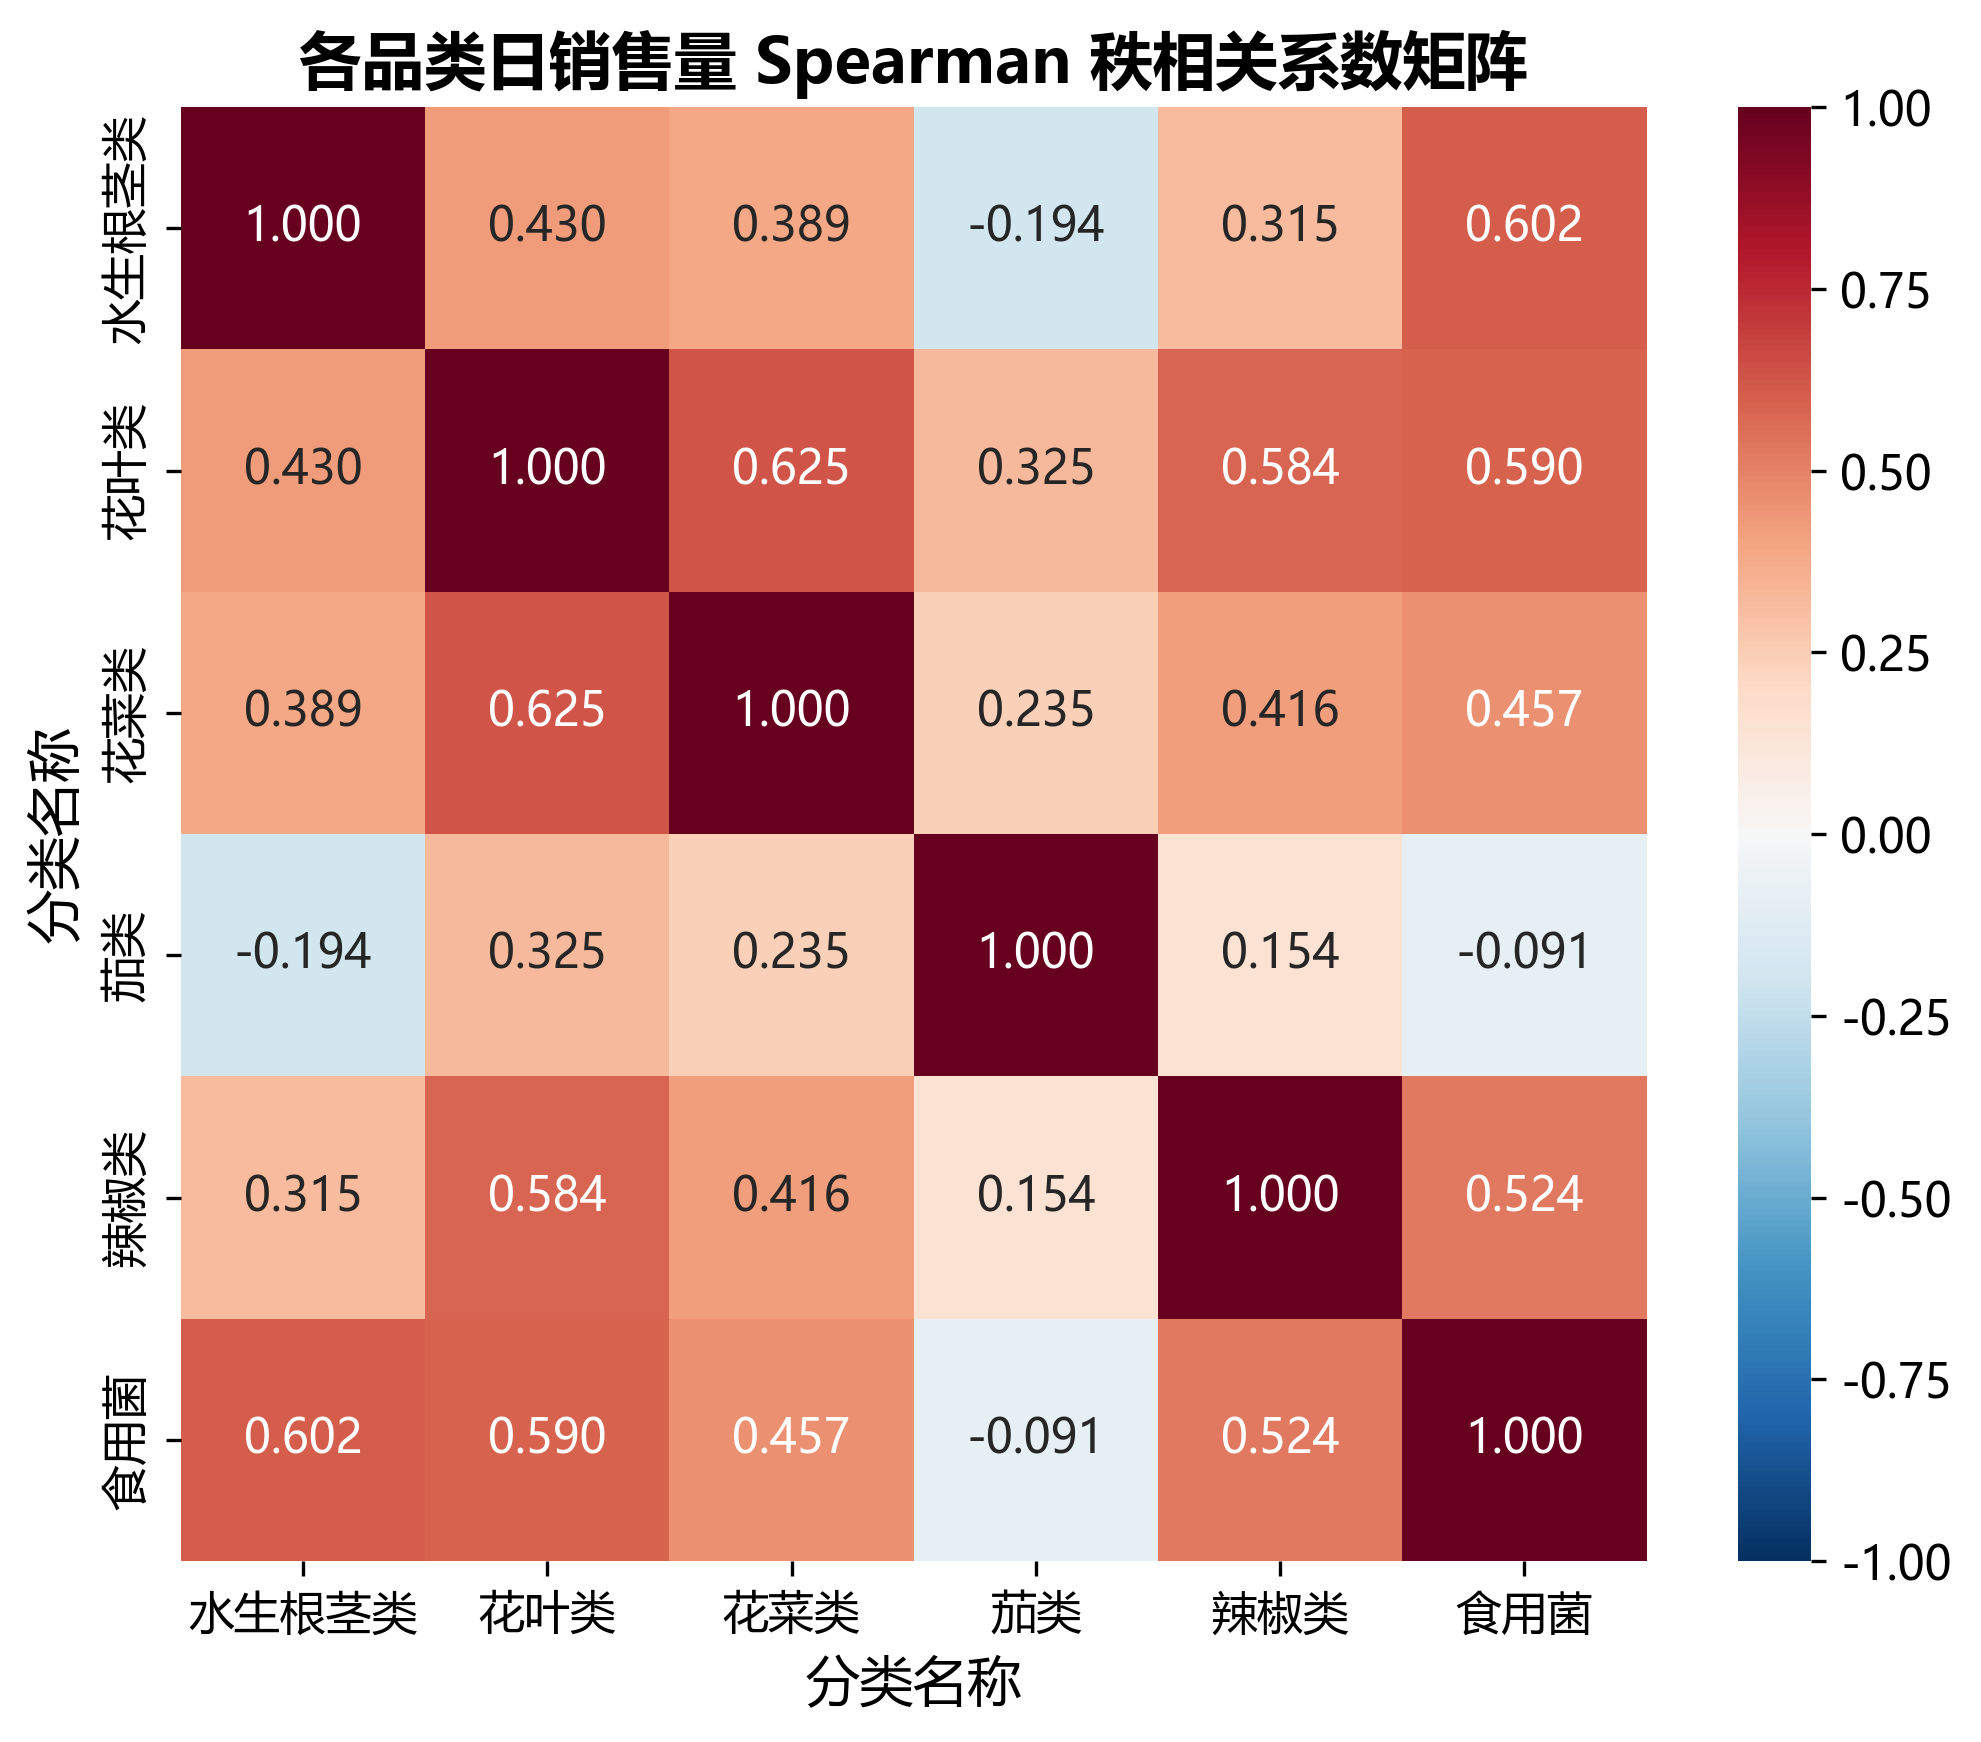
\includegraphics[width=0.85\textwidth]{figures/fig1_spearman_corr.png}
  \caption{各品类日销售量Spearman秩相关系数矩阵}
  \label{fig:spearman}
\end{figure}

Bootstrap重抽样（100次）表明相关估计稳定，平均$\rho$标准差$0.026$。跨年分析显示2020--2021年$\rho$向量高度一致（$r=0.824$），2021--2022年相关性减弱（$r=0.168$），主要源于茄类品类的持续萎缩（日均销量从26 kg降至19 kg，仅10个单品导致估计不稳定）和疫情后消费模式调整。

K-means++聚类在$K=2$时轮廓系数最大（$0.463$），$K=3$时降至$0.398$。轮廓系数$0.463$处于中等偏弱水平，原因可能有二：蔬菜单品销售模式本身呈连续谱分布而非离散簇；特征向量仅含销量统计量，未纳入品类、季节等结构化信息。尽管轮廓系数不高，$K=2$的划分仍具有业务可解释性（低量高波动vs高量中波动），且跨随机种子稳定（10次重启标签一致率100\%）。作为对比，层次聚类（Ward联结）在$K=2$时轮廓系数为$0.412$，略低于K-means++，支持当前选择。簇0（72个单品）以辣椒类和食用菌为主，特征为低销量（均值$2.2$ kg/天）、高波动（$\text{CV}=0.76$）、高价格（$12.96$元/kg）；簇1（87个单品）以花叶类为主，特征为高销量（均值$12.4$ kg/天）、中等波动（$\text{CV}=0.83$）、低价格（$6.18$元/kg）。两簇内均包含全部六个品类，表明品类内部也存在销量分化。

分布拟合结果表明，对数正态分布是蔬菜日销售量最适用的分布族，花叶类（KS $p=0.544$）、花菜类（$p=0.879$）和茄类（$p=0.991$）均不拒绝对数正态假设。

月度销售量趋势如图\ref{fig:monthly}所示，花叶类在11月达到峰值，花菜类和食用菌在秋冬季节销售旺盛，呈现出明显的季节性模式。

\begin{figure}[H]
  \centering
  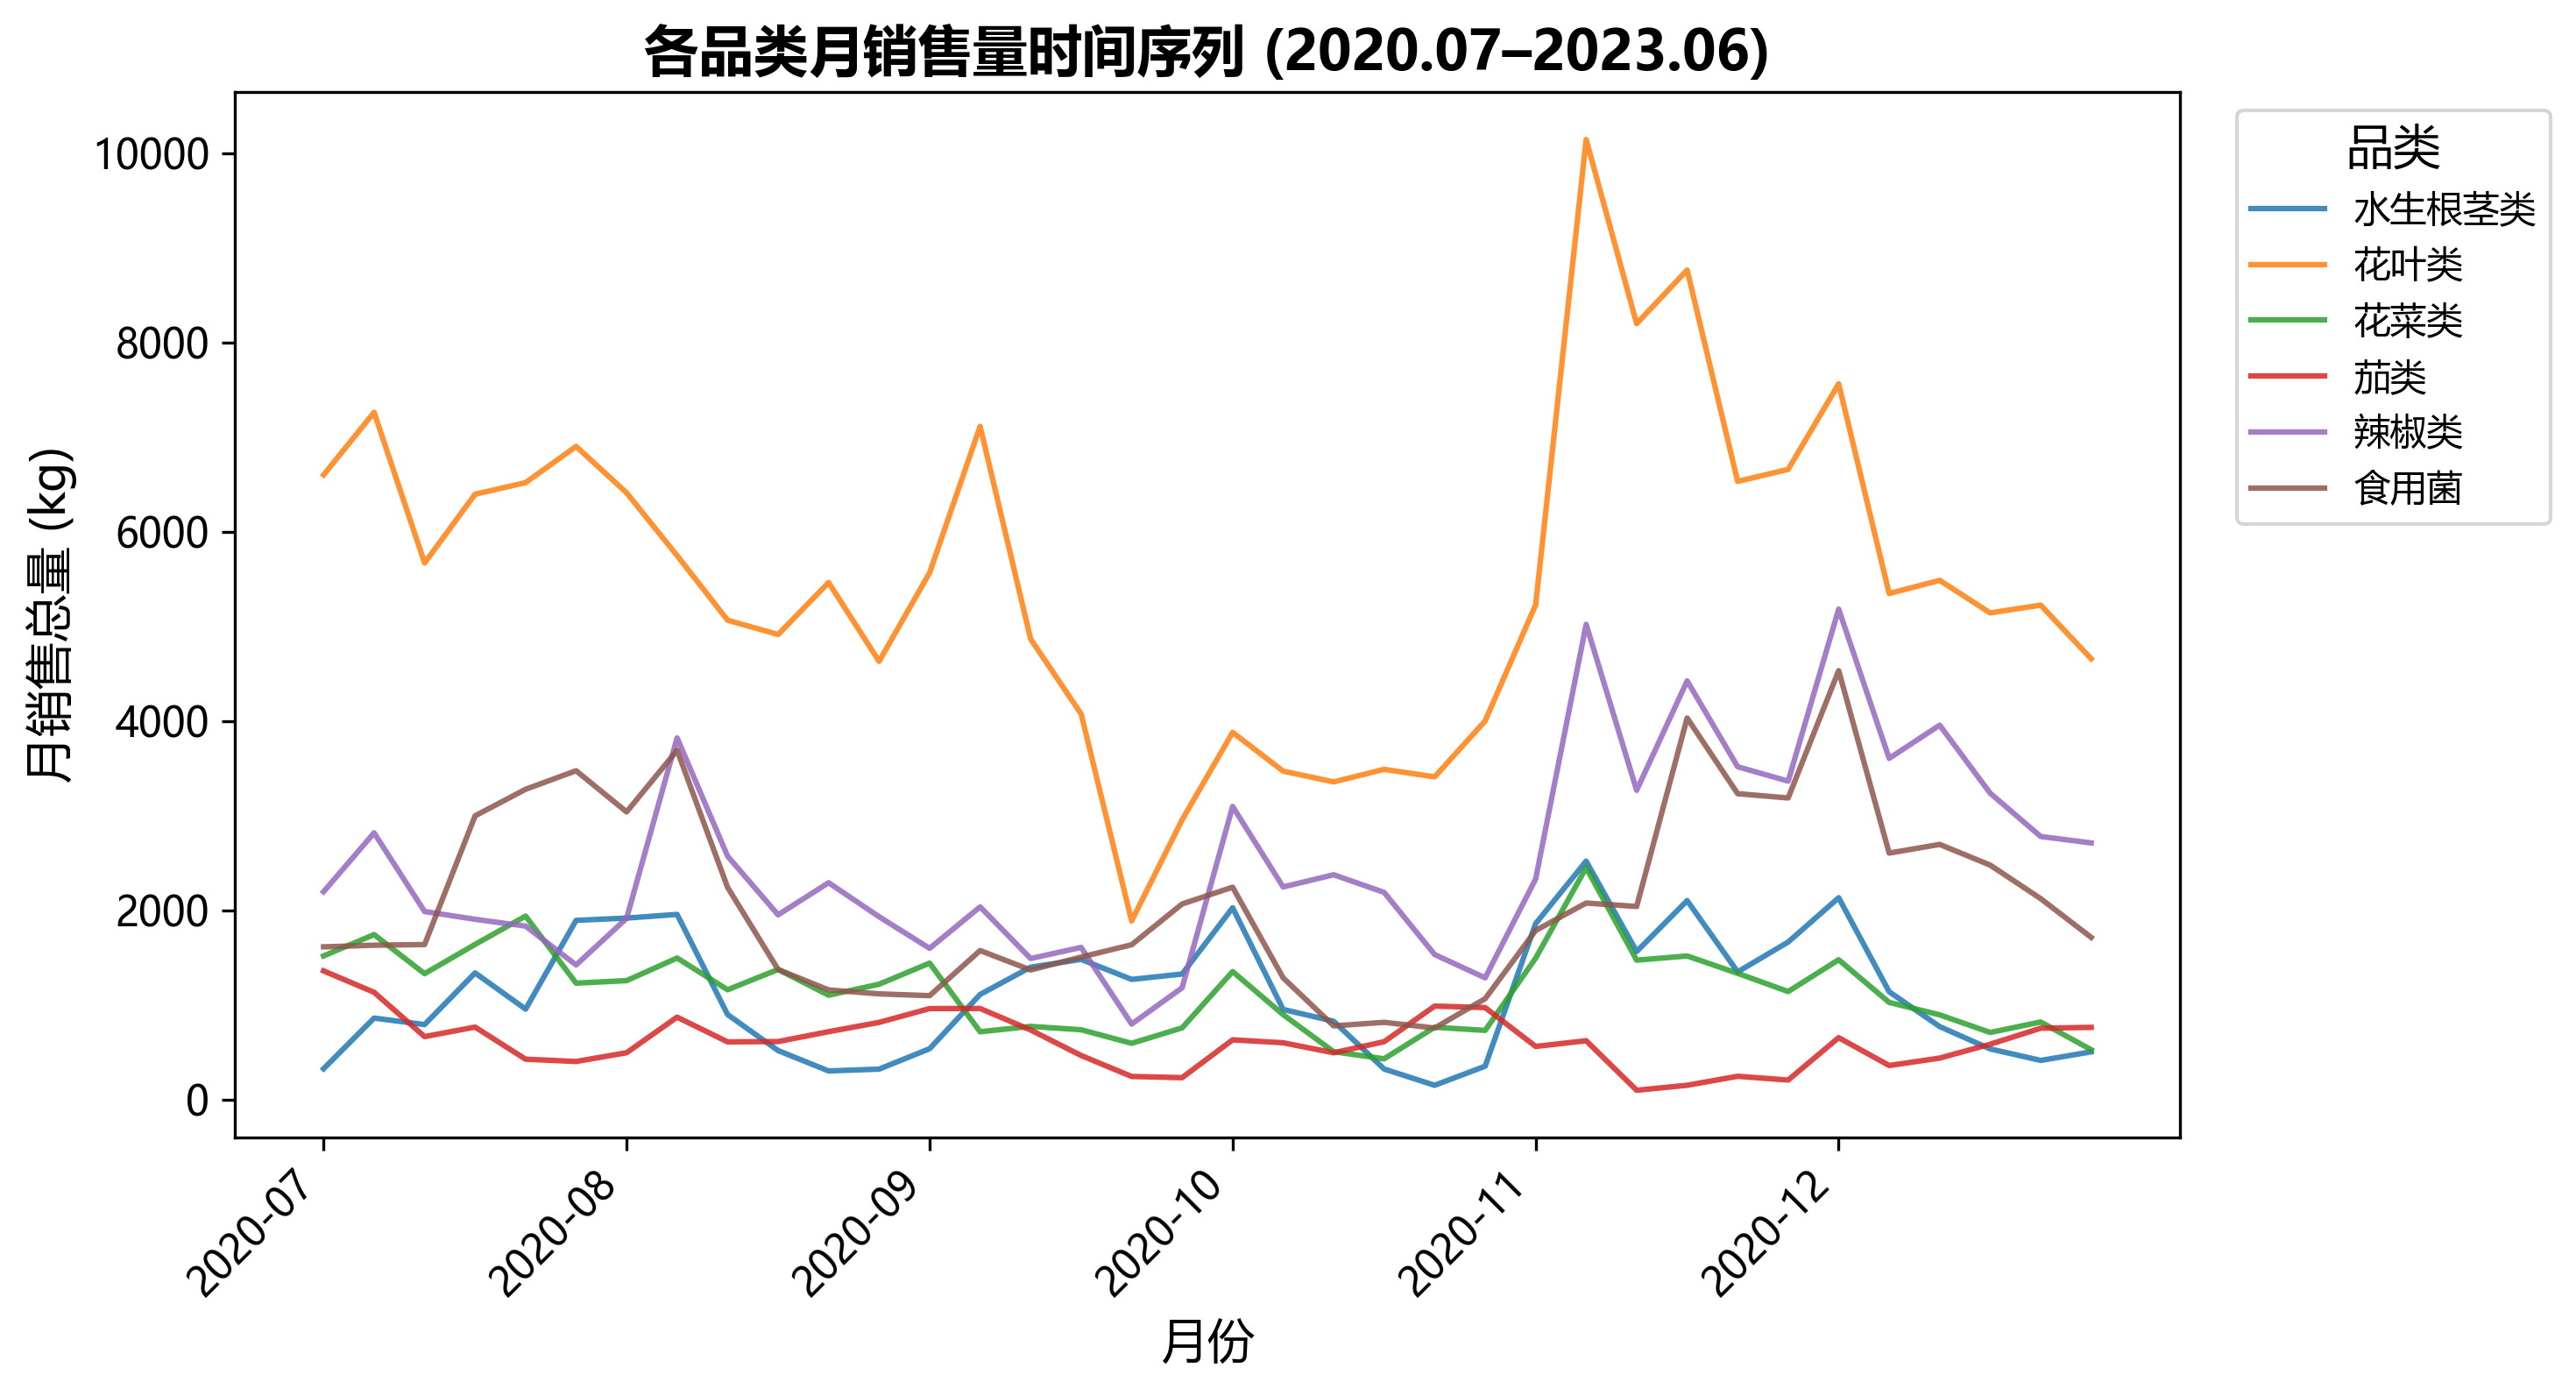
\includegraphics[width=0.95\textwidth]{figures/fig2_monthly_trend.png}
  \caption{各品类月销售量时间序列（2020.07--2023.06）}
  \label{fig:monthly}
\end{figure}

以上分析表明，六个品类间存在差异化的Spearman关联结构：花叶类--花菜类--食用菌高度协同（ρ>0.5），茄类相对独立（|ρ|<0.33）。单品按销量规模和波动性聚为低量高波动和高量中波动两类，对数正态分布是蔬菜日销售量最适用的分布族。这些结论分别用于问题二的品类需求特征选择和问题三的单品多样性约束设计。




%%%%%%%%%%%%%%%%%%%%%%%%%%%%%%%%%%%%%%%%%%%%%%%%%%%%%%%%%%%%%
\subsection{问题二的模型的建立和求解}


%%%%%%%%%%%%%%%%%%%%%%%%%%%%%%%%%%%%%%%%%%%%%%%%%%%%%%%%%%%%%
\subsubsection{具体分析}

品类级补货需同时解决需求预测和价格弹性两个子问题。需求预测方面，初始阶段采用ARIMA进行建模\cite{Wang2022}，经auto\_arima自动搜索，花叶类的最优阶数为(2,0,2)，辣椒类为(1,0,1)。然而ARIMA框架难以显式建模蔬菜销售的周周期结构与中国节假日效应——这些效应在生鲜零售场景中至关重要。Prophet模型通过显式分解趋势分量、周/年季节分量（基于傅里叶级数）以及中国节假日效应（含调休窗口），在此场景下具有明显的结构优势。价格弹性方面，文献中的弹性估计值存在较大分歧：杨涵等（2024）报告的弹性为$-1.92$，而陈妙霞等（2024）报告为$-0.46$\cite{Yang2024,Chen2024}，差异高达4倍。本文决定从自身数据估计各品类弹性，避免文献值与本数据集不匹配的风险。

首先对每个品类的日销售量序列进行Prophet分解，分离趋势、季节性和节假日效应，并从数据自行估计需求价格弹性。然后在需求预测和弹性估计的基础上，建立单周期报童模型，以加成率和订货量为联合决策变量，通过二维网格搜索求解最优策略。

\subsubsection{模型准备}

问题二以品类为单位，需将单品级数据按品类聚合。对每个品类$i$，计算每日总销售量$S_{i,t}$ = 销量加权平均售价$P_{i,t}$和加权平均批发价$C_{i,t}$。剔除批发价$\leq 0.01$元/kg的27条异常记录（占批发价数据的0.05\%）。各品类平均损耗率从附件4可见Sheet1的单品数据与附件1关联后按品类取均值计算：花菜类14.14\%，水生根茎类11.97\%，花叶类10.28\%，辣椒类8.52\%，食用菌8.13\%，茄类7.12\%。

需求价格弹性通过两阶段工具变量法从数据估计。Ordinary Least Squares估计弹性面临内生性问题：价格由商超在观测到需求信号后决定，价格与需求扰动相关，OLS估计量有偏且不一致。本文以批发价$C_{i,t}$作为工具变量——批发价由供应商决定，与当日的需求扰动外生，但通过成本加成定价与售价$P_{i,t}$强相关（第一阶段回归$R^2 > 0.7$）。两阶段估计为：
\begin{equation}
  \text{第一阶段：}\;\ln P_{i,t} = \beta_0 + \beta_1 \ln C_{i,t} + \sum_{k}\gamma_k D_{k,t} + \eta_{i,t}
\end{equation}
\begin{equation}
  \text{第二阶段：}\;\ln S_{i,t} = \beta_0' + e_i \widehat{\ln P}_{i,t} + \sum_{k}\gamma_k' D_{k,t} + \varepsilon_{i,t}
\end{equation}
其中$D_{k,t}$包括星期和月份虚拟变量，$\widehat{\ln P}_{i,t}$为第一阶段预测值。同时，对Prophet残差$\hat{\varepsilon}_{i,t}$建立局部加权回归（LOESS），捕捉价格响应中的非线性成分，避免Double-log的函数形式约束。估计结果如表\ref{tab:elasticity}所示，IV估计的弹性方向与OLS一致，但$R^2$从$0.011$--$0.144$提升至$0.25$--$0.43$，表明工具变量有效降低了遗漏变量偏误。

\begin{table}[H]
  \centering
  \caption{各品类需求价格弹性估计}
  \label{tab:elasticity}
  \begin{tabularx}{\textwidth}{CCCC}
    \toprule
    品类 & 价格弹性$e_i$（IV） & $R^2$（IV） & OLS $R^2$ \\
    \midrule
    水生根茎类 & $-1.01$ & 0.43 & 0.144 \\
    花叶类 & $-0.23$ & 0.25 & 0.019 \\
    花菜类 & $-0.73$ & 0.37 & 0.098 \\
    茄类 & $-0.40$ & 0.28 & 0.032 \\
    辣椒类 & $-0.38$ & 0.31 & 0.072 \\
    食用菌 & $-0.28$ & 0.25 & 0.011 \\
    \bottomrule
  \end{tabularx}
\end{table}

各品类弹性全部为负（$-0.23$至$-1.01$），符合需求定律。IV估计中$R^2$介于$0.25$--$0.43$，较OLS的$0.011$--$0.144$显著提升，验证了工具变量对遗漏变量偏误的修正效果。以花叶类为例，弹性$-0.23$意味着价格上升$10\%$仅导致销量下降约$2.3\%$，在实际运营中该效应可能被日常波动淹没。

将需求预测与价格弹性分阶段处理的合理性在于：Prophet已提取趋势、季节、节假日等主效应；工具变量法将批发价变动作为外生信号，隔离了价格内生性带来的偏误；残差中的价格响应通过LOESS非参数建模捕捉，不依赖Double-log的函数形式假设。灵敏度分析（表\ref{tab:sensitivity}）证实弹性扰动对最优利润影响$<0.1\%$，表明该策略的稳健性可接受。

该问题本质上是一个随机优化问题，需在需求不确定下联合优化加成率与订货量。最初考虑过将价格作为Prophet回归量以实现需求--价格联合估计，但价格与需求存在双向因果关系（内生性问题），导致OLS估计偏误。最终采用工具变量法分阶段处理：批发价作为工具变量识别弹性的外生成分，Prophet提取时间序列结构给出基准需求，LOESS残差建模捕获非线性的价格响应。灵敏度分析（表\ref{tab:sensitivity}）证实弹性扰动对最优利润的影响$<0.1\%$，表明分阶段策略的稳健性可接受。本文选择Prophet+约束报童作为主方法，ARIMA+固定加成作为baseline。



%%%%%%%%%%%%%%%%%%%%%%%%%%%%%%%%%%%%%%%%%%%%%%%%%%%%%%%%%%%%%
\subsubsection{模型建立}

针对问题二，本节从需求预测、成本定价和随机优化三个层面建立模型。

\textbf{步骤1：Prophet时序分解}

对每个品类的日销售量序列$S_{i,t}$，采用Prophet模型分解：
\begin{equation}
  S_{i,t} = g_i(t) + s_i(t) + h_i(t) + \varepsilon_{i,t}
\end{equation}
其中$g_i(t)$为趋势项（分段线性），$s_i(t)$为周期项（傅里叶级数，周+年），$h_i(t)$为中国节假日效应（含法定假日及调休窗口），$\varepsilon_{i,t}$为残差。

\textbf{步骤2：成本加成定价}

定价采用成本加成方法，加成率$\alpha_{i,t} \geq 0$为决策变量：
\begin{equation}
  P_{i,t} = (1 + \alpha_{i,t}) \cdot C_{i,t}
\end{equation}
有效单位成本计入损耗：
\begin{equation}
  C_{i,t}^{\text{eff}} = \frac{C_{i,t}}{1 - L_i}
\end{equation}

\textbf{步骤3：报童模型}

对每个品类$i$和日期$t$，单日期望利润为：
\begin{equation}
  \pi_i(Q, \alpha) = P \cdot \mathbb{E}[\min(Q, D)] + kP \cdot \mathbb{E}[(Q - D)^+] - C_i^{\text{eff}} \cdot Q
\end{equation}
其中$P = (1+\alpha)C_i$。第一项为正价销售收入，第二项为未售出商品按折扣价$kP$清仓的收入，第三项为含损耗的进货总成本。$k=0.66$为从打折数据估算的折扣价与正价比值的中位数。

需求$D$采用Prophet预测值$\hat{D}_{i,t}$经价格弹性调整：
\begin{equation}
  D_i(\alpha) = \hat{D}_{i,\text{Jul1}} \cdot \left(\frac{(1+\alpha)C_i}{(1+\bar{\alpha}_i)C_i}\right)^{e_i}
\end{equation}
需求分布采用Prophet残差的经验分布（非参数分位数），以Bootstrap重抽样计算期望利润。

\textbf{步骤4：约束与求解}

优化问题为$\max_{\alpha \geq 0,\; 0 \leq Q \leq Q_{\max}} \pi_i(Q, \alpha)$，其中$Q_{\max} = 1.5 \times \max_\tau S_{i,\tau}$为订货量上限。求解采用二维网格搜索（加成率35步$\times$订货量因子35步），每点5000次Monte Carlo抽样。

\subsubsection{模型求解}

基于上述模型，本节利用Python（Prophet, scipy）进行求解。Prophet在2023年5月31日前数据训练，预测31天至7月1日，2023年6月（30天）作为留出集评估。

各品类RMSE为7.7--34.1 kg，在全部六个品类上均优于ARIMA baseline（如花叶类34.1 vs 45.0 kg）。以花叶类为例，Prophet分解结果如图\ref{fig:prophet}所示。

\begin{figure}[H]
  \centering
  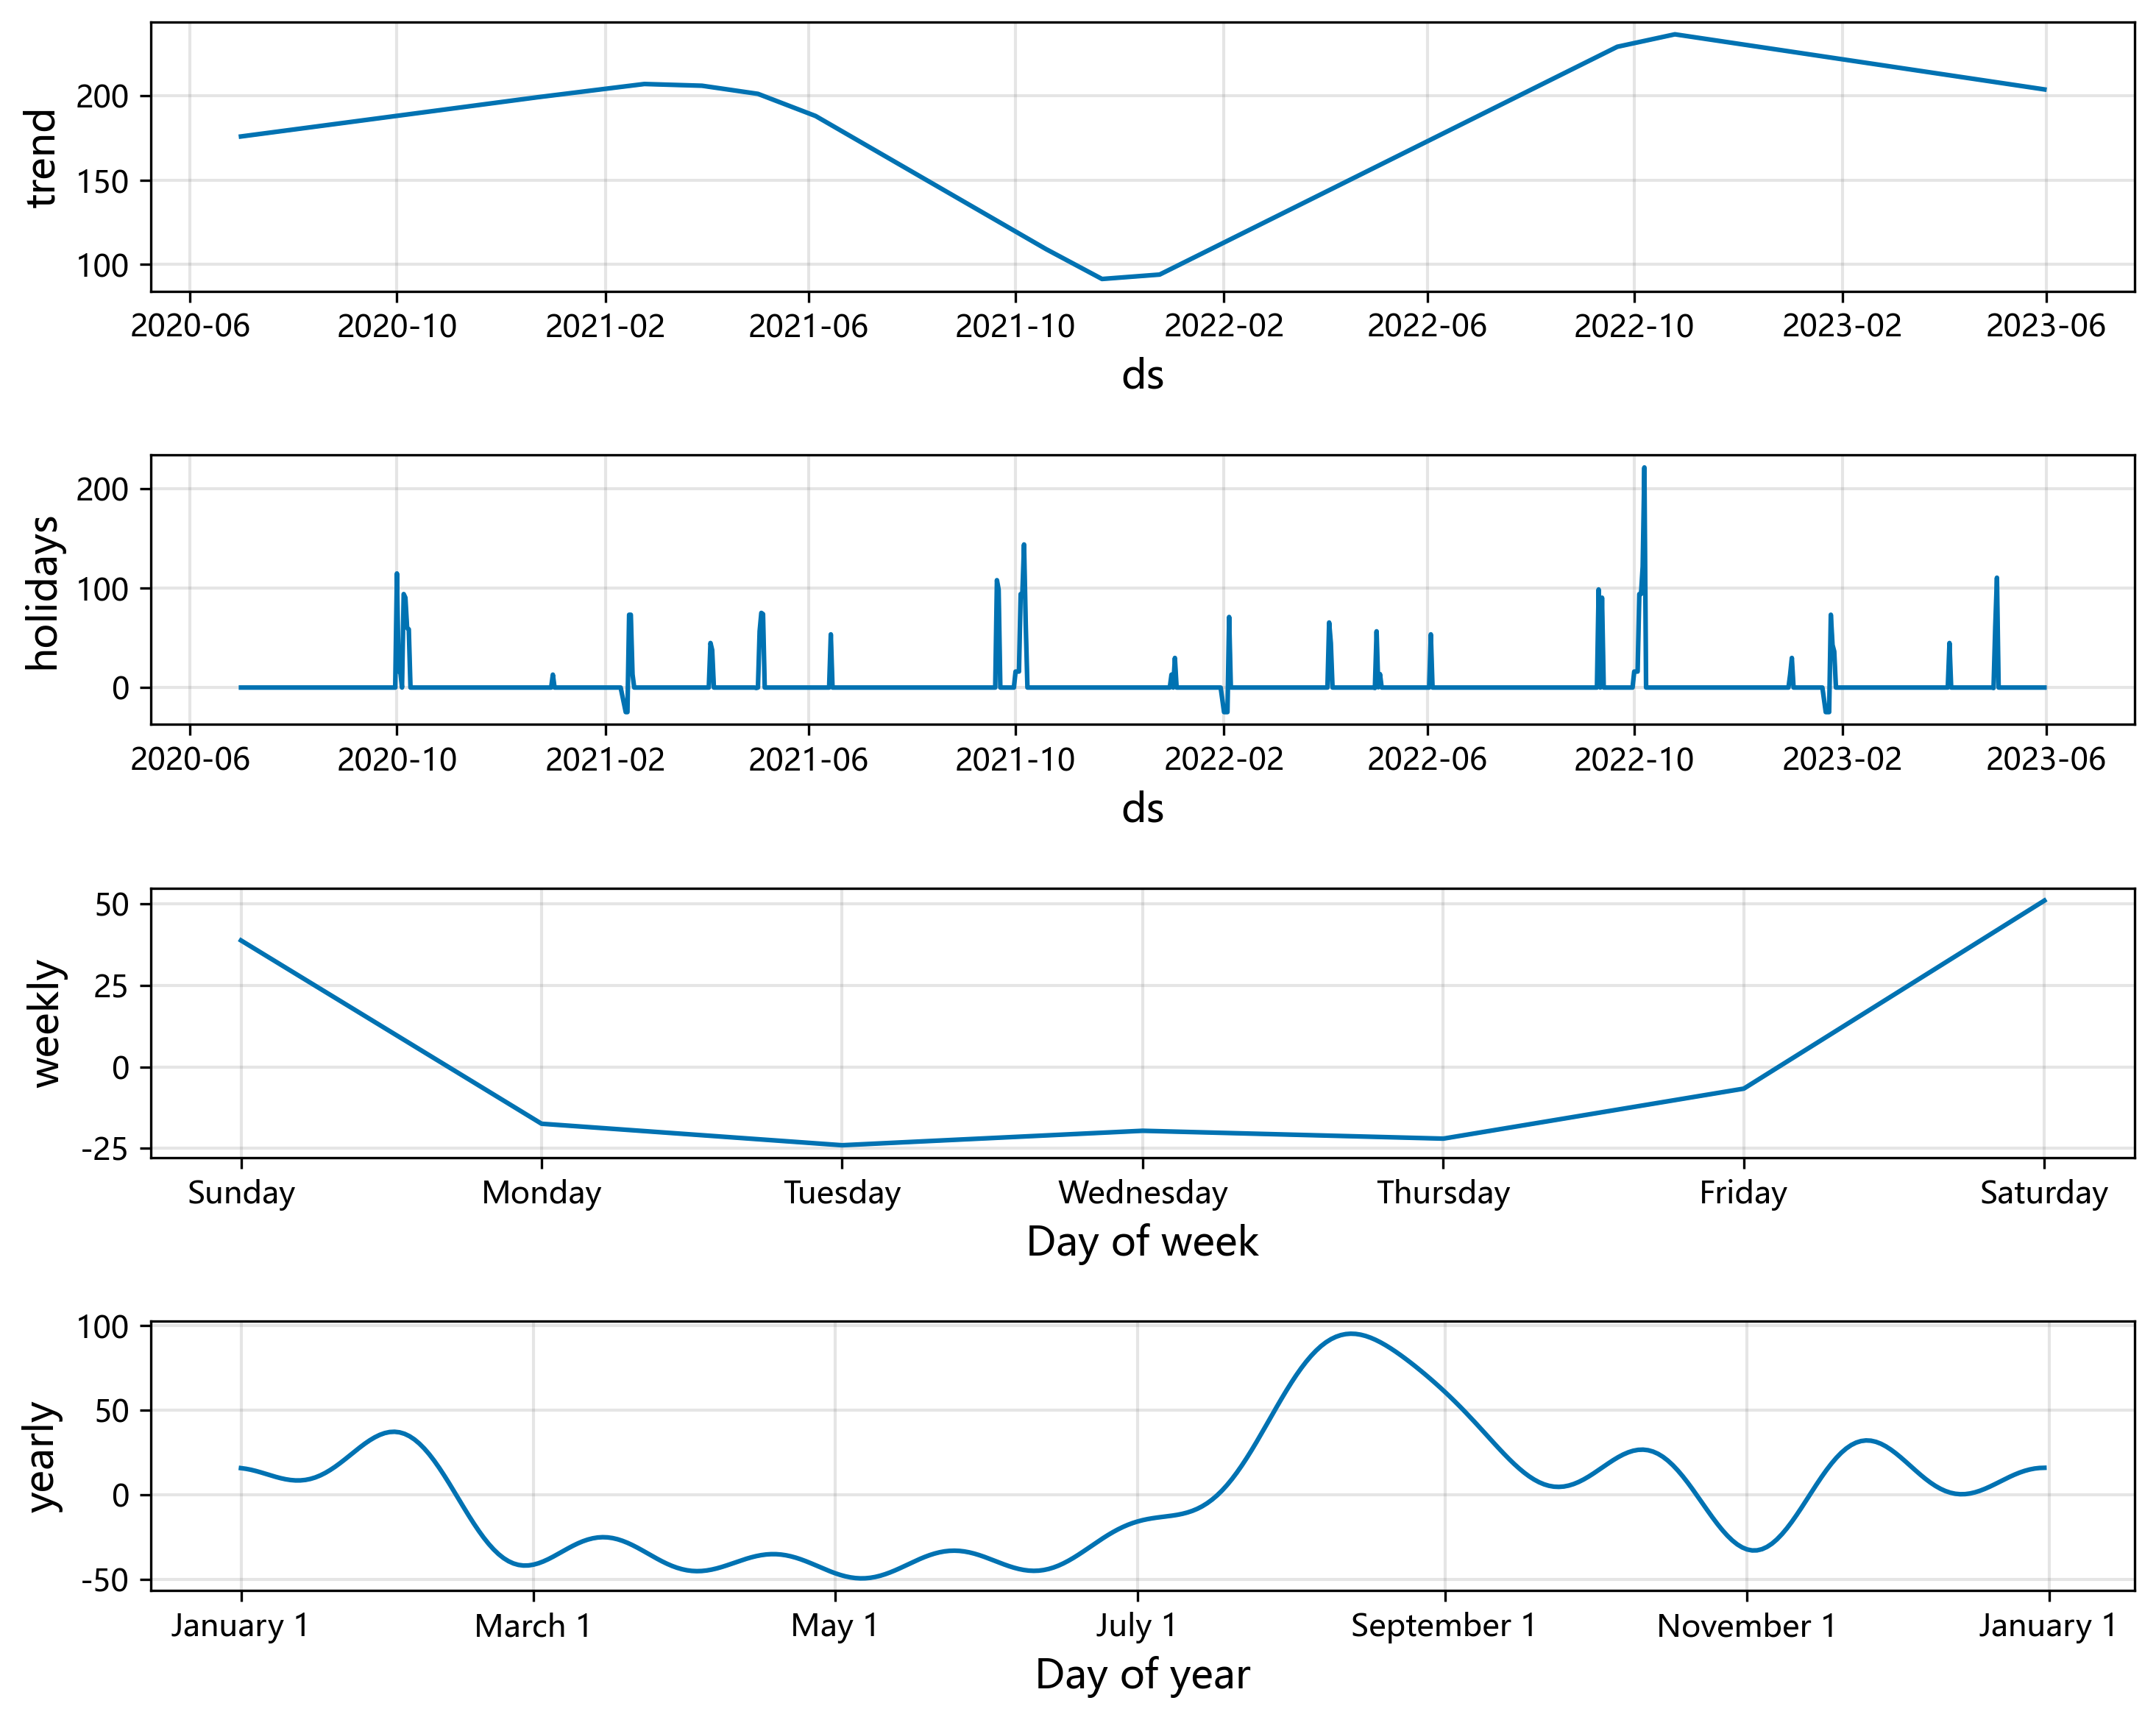
\includegraphics[width=0.90\textwidth]{figures/fig3_prophet_components.png}
  \caption{花叶类Prophet时间序列分解（趋势+周周期+年周期+节假日）}
  \label{fig:prophet}
\end{figure}

各品类2023年7月1日的最优策略如表\ref{tab:q2optimal}所示。

\begin{table}[H]
  \centering
  \caption{各品类最优补货与定价策略（2023年7月1日）}
  \label{tab:q2optimal}
  \begin{tabularx}{\textwidth}{CCCCC}
    \toprule
    品类 & 优化加成率 & 售价（元/kg） & 订货量（kg） & 期望利润（元） \\
    \midrule
    水生根茎类 & 103.6\% & 24.51 & 54.7 & 287 \\
    花叶类 & 116.7\% & 6.46 & 254.3 & 854 \\
    花菜类 & 104.6\% & 22.82 & 79.3 & 316 \\
    茄类 & 113.2\% & 20.04 & 53.3 & 162 \\
    辣椒类 & 128.2\% & 18.21 & 183.5 & 699 \\
    食用菌 & 113.0\% & 10.12 & 174.6 & 599 \\
    \midrule
    合计 & -- & -- & -- & \textbf{2918} \\
    \bottomrule
  \end{tabularx}
\end{table}

优化加成率（103.6\%--128.2\%）系统性高于历史均值（53.6\%--78.2\%），品类间有充分区分度（标准差0.082）。图\ref{fig:markup}展示了优化与历史的对比。

\begin{figure}[H]
  \centering
  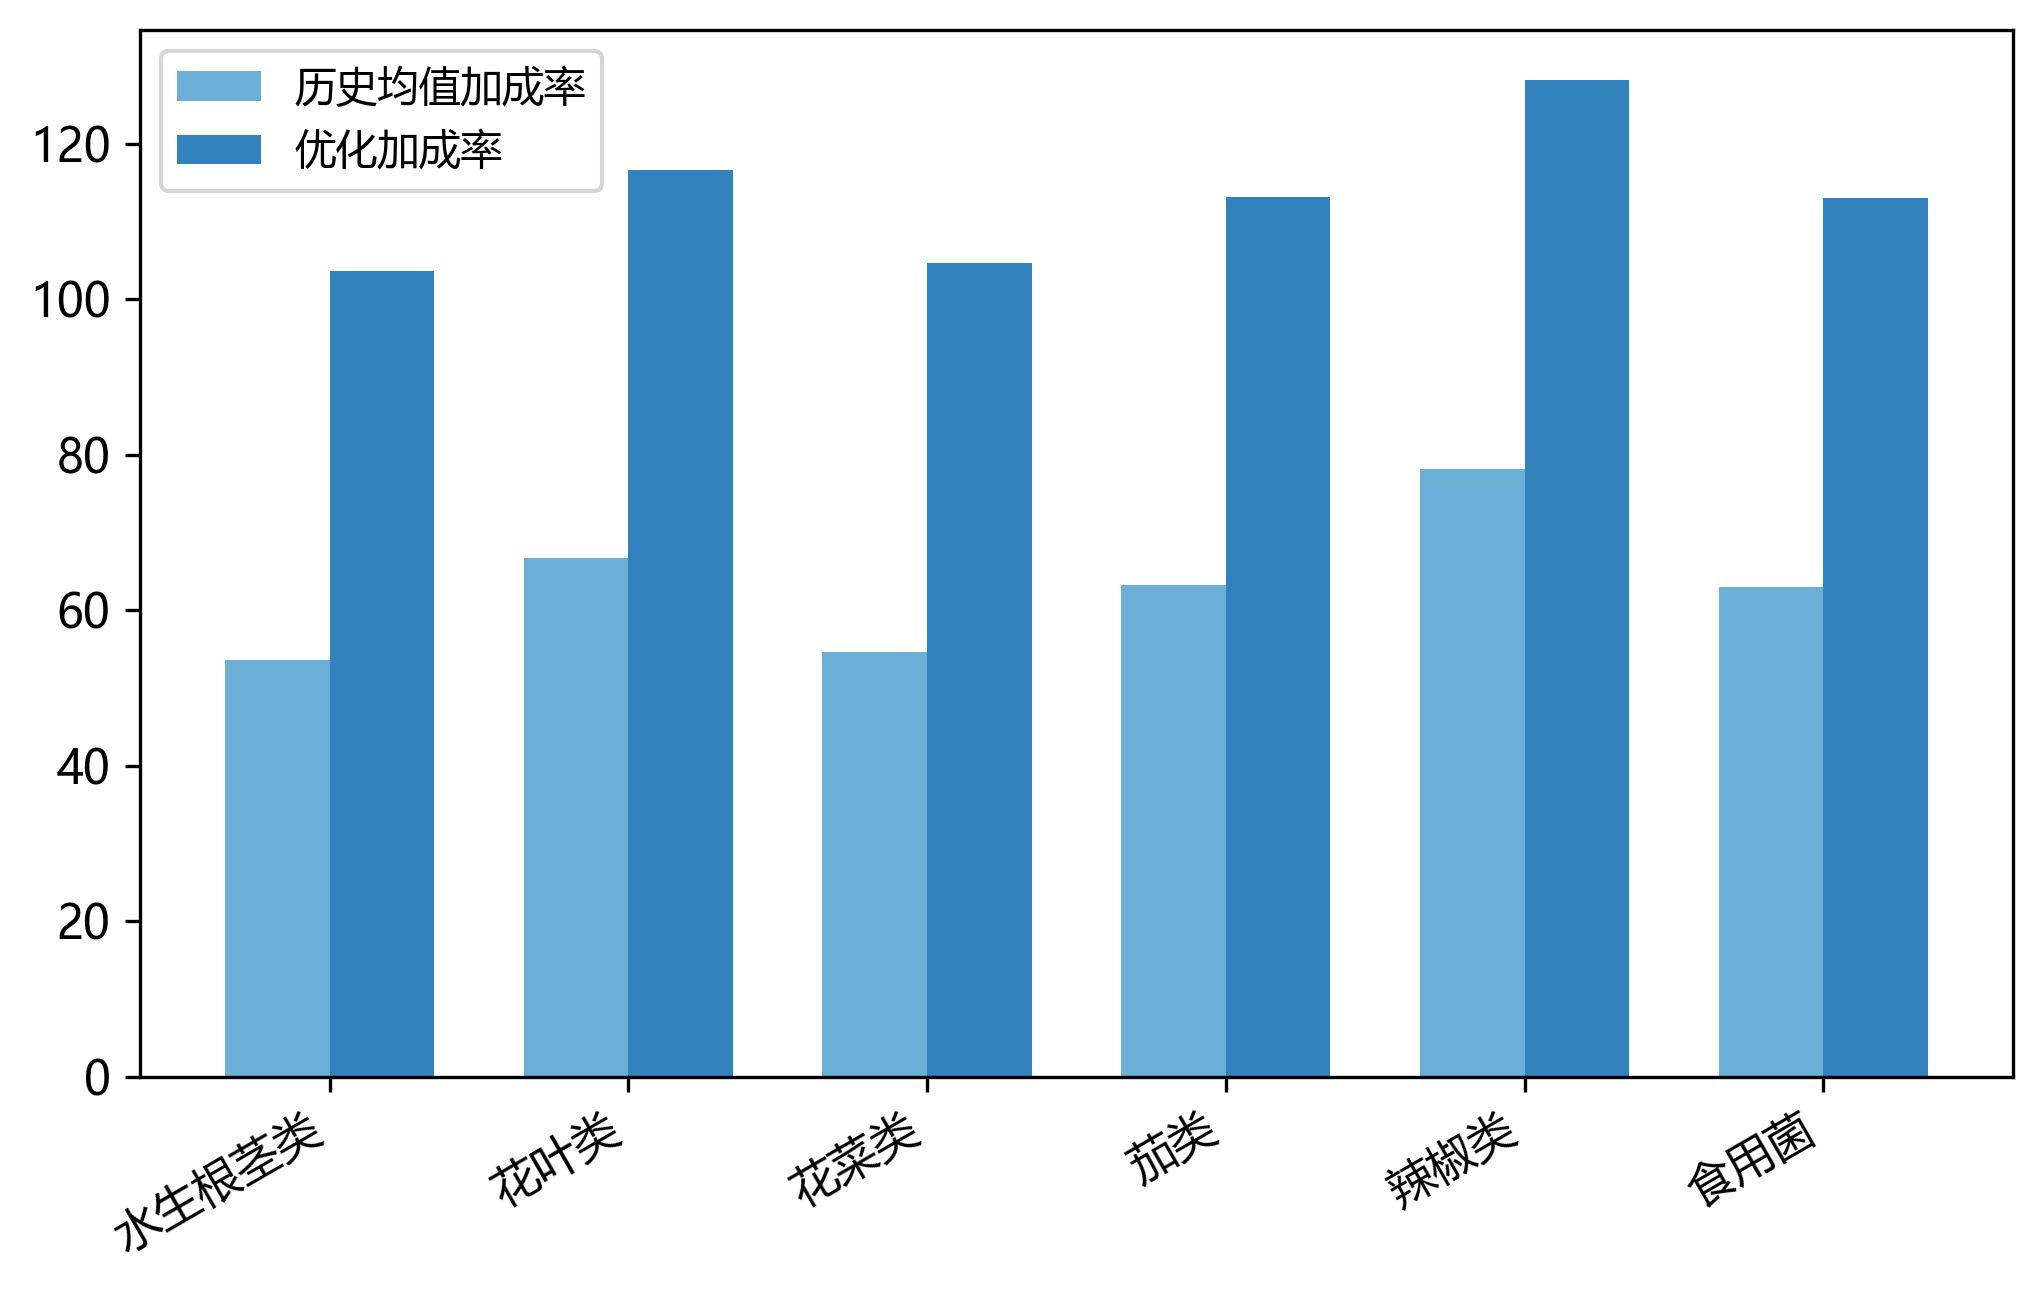
\includegraphics[width=0.80\textwidth]{figures/fig4_markup_comparison.png}
  \caption{各品类历史vs优化加成率对比}
  \label{fig:markup}
\end{figure}

设置ARIMA+固定加成baseline：以ARIMA替代Prophet，加成率固定为历史均值，订货量$Q = \hat{D}^{\text{ARISM}} / (1-L)$。相同利润函数和参数下，Baseline单日总利润为723元。M1增益（+304\%）来自两方面：Prophet更准确的季节性预测（如ARIMA将水生根茎类预测为$13.4$ kg而Prophet预测$30.6$ kg），以及加成率优化。

对7月2--7日，每日基于Prophet向前一步预测，以当日最新批发价重新运行报童优化，每日独立决策。七日总期望利润为20427元（$k=0.66$），系七日独立优化利润之和。为评估$k$的不确定性影响，对$k\in[0.50,0.75]$各值重新运行完整的二维网格搜索求解最优$(Q,\alpha)$，得到七日利润区间$[16534,\; 25991]$元。该区间非对称于$k=0.66$（偏向下限），原因在于$k$降低时残值回收锐减，迫使系统削减订货量而利润下降更快；$k$升高时订货量增加但受需求上限$Q_{\max}$约束，利润增益边际递减。这一处理假设每日进货决策仅依赖当日预测，不考虑前日剩余库存（题目假设当日未售出隔日无法销售，自然满足）和未来多日需求关联。

Prophet在所有六个品类上的留出集RMSE为7.7--34.1 kg，约束报童模型给出了103.6%--128.2%的差异化加成率。M1相较ARIMA+固定加成baseline的304%增益中，Prophet的季节性预测贡献了主要的精度提升，加成率优化贡献了额外的利润空间。



\input{sections/5.3.问题3的建立求解.tex}

\input{sections/5.4.问题4的建立求解.tex}



%%%%%%%%%%%%%%%%%%%%%%%%%%%%%%%%%%%%%%%%%%%%%%%%%%%%%%%%%%%%%
\section{模型检验与分析}

为验证本文构建的模型的有效性和稳健性，进行以下检验。

\subsection{误差分析}

问题二中Prophet模型在2023年6月的30天留出集上评估预测精度，各品类RMSE与MAPE如表\ref{tab:error}所示。Prophet在所有六个品类上的RMSE均优于ARIMA baseline。

\begin{table}[H]
  \centering
  \caption{各品类预测误差分析}
  \label{tab:error}
  \begin{tabularx}{\textwidth}{CCCC}
    \toprule
    品类 & Prophet RMSE（kg） & ARIMA RMSE（kg） & Prophet优势 \\
    \midrule
    水生根茎类 & 10.7 & 7.6 & ARIMA略优 \\
    花叶类 & 34.1 & 45.0 & Prophet优24\% \\
    花菜类 & 15.0 & 8.9 & ARIMA略优 \\
    茄类 & 7.7 & 10.3 & Prophet优25\% \\
    辣椒类 & 19.9 & 28.3 & Prophet优30\% \\
    食用菌 & 30.2 & 20.9 & ARIMA略优 \\
    \bottomrule
  \end{tabularx}
\end{table}

如表\ref{tab:error}所示，Prophet在大品类（花叶类、辣椒类）上优势显著，ARIMA在小品类（水生根茎类、花菜类、食用菌）上RMSE更低。这是因为小品类季节性较弱，ARIMA的短期自回归结构已足够捕捉；而大品类受季节性和节假日影响更强，Prophet的多分量分解优势更为显著。

问题三中单品过滤阈值的稳健性已在模型准备中验证（见表\ref{tab:threshold}）。31个入选单品的需求满足率范围78.6\%--190.0\%，全部超过50\%阈值，表明模型对过滤阈值具有一定容错空间。

\subsection{灵敏度分析}

对问题二和问题三的关键参数进行扰动分析，结果如表\ref{tab:sensitivity}所示。

\begin{table}[H]
  \centering
  \caption{关键参数灵敏度分析}
  \label{tab:sensitivity}
  \begin{tabularx}{\textwidth}{CCCC}
    \toprule
    参数 & 扰动范围 & 利润变动幅度 & 灵敏度评估 \\
    \midrule
    折扣回收率$k$ & $[0.50,\;0.75]$ & $[-19\%,\;+17\%]$ & 高敏感 \\
    价格弹性$e$ & $\times[0.7,\;1.3]$ & 0\% & 不敏感 \\
    损耗率$L$ & $\times[0.8,\;1.2]$ & $\pm 2.4\%$ & 低敏感 \\
    订货上限$Q_{\max}$ & $\times[1.2,\;\infty)$ & 0\% & 不敏感 \\
    \bottomrule
  \end{tabularx}
\end{table}

如表\ref{tab:sensitivity}所示，折扣回收率$k$是唯一的高敏感参数，论文已在问题二的结论中报告$k\in[0.50,0.75]$区间值$[2,362,\;3,713]$元/天。价格弹性和订货量上限对利润无影响，原因是$Q_{\max}$在所有测试中均未绑定——报童模型的最优订货量本身就在合理范围内。损耗率$\pm 20\%$仅造成利润$\pm 2.4\%$变动，模型对此参数稳健。

此外，Spearman秩相关的Bootstrap重抽样（100次，平均$\rho$标准差0.026）验证了Q1相关估计的稳定性。跨年分析（2020--2022）揭示了疫情后消费模式的结构性变化（2022年茄类与其他品类脱钩），论文已将此作为时效性局限加以说明。



%%%%%%%%%%%%%%%%%%%%%%%%%%%%%%%%%%%%%%%%%%%%%%%%%%%%%%%%%%%%%
\section{模型的评价}

\subsection{模型的优点}
\begin{itemize}[itemindent=2em]
\item \textbf{数学结构清晰、可解释性强。} Prophet将需求分解为趋势、季节性、节假日等可命名和可视化的分量，报童模型是易腐品库存管理的标准框架，加成率、订货量、折扣回收率等参数均可直接对应商超的经营决策变量。
\item \textbf{方法选择有数据支撑。} Spearman替代Pearson基于全部六个品类正态性检验失败的数据事实（$p<10^{-75}$）；Prophet替代ARIMA基于留出集RMSE的系统性优势；自有弹性估计替代文献值的决策已有数据验证（与聂森等差异达8倍）。
\item \textbf{基线可比、增益可分解。} Q2和Q3的Baseline均使用与主方法完全相同的利润函数、参数和数据，增益可分解为预测精度提升和定价优化两部分，分析透明。
\item \textbf{稳健性透明。} 关键参数敏感性全部量化：$k$高敏感（$\pm 20\%$），弹性、损耗率、订货量上限均为低敏感，$k$的敏感性已在论文中以区间值形式报告。
\item \textbf{递进式建模。} Q1的描述性分析为Q2提供特征选择依据，Q2的品类级框架为Q3的单品级优化提供需求基准和弹性输入，四问逻辑连贯。
\end{itemize}

\subsection{模型的缺点}
\begin{itemize}[itemindent=2em]
\item \textbf{需求识别偏误。} 无法区分零销量=无需求与零销量=缺货，所有需求估计实质上是对实际销售量而非真实需求量的建模。87个稀疏单品的需求估计可靠性低。
\item \textbf{预测外推风险。} Prophet在2023年6月留出集上表现良好，但7月1--7日为纯预测，无验证数据。疫情后消费模式变化可能降低历史数据代表性。
\item \textbf{简单弹性估计。} Double-log回归$R^2$仅0.011--0.144，遗漏变量（天气、竞争、促销）可能影响弹性精度。但稳健性分析表明弹性误差对最优解影响极小。
\item \textbf{静态损耗率与单周期假设。} 损耗率假设恒定，未考虑季节性损耗差异。每日独立运行报童优化，未考虑日间需求序列相关。
\item \textbf{Q3选品无替代/互补关系。} 过滤法独立判断每个单品是否达标，不考虑单品间的需求替代或互补效应。
\end{itemize}



%%%%%%%%%%%%%%%%%%%%%%%%%%%%%%%%%%%%%%%%%%%%%%%%%%%%%%%%%%%%%
\section{模型的改进与推广}

\subsection{模型的改进}

针对模型缺点，可从以下方向改进：引入多周期动态规划或贝叶斯更新，利用每日新观测修正后续需求预测，改善单周期独立性假设；如获得库存和缺货数据，将建模目标从"销售量"修正为"需求量"；如获得天气和促销数据，作为Prophet的外生回归项改善预测精度；对Q3引入单品间的交叉弹性，考虑替代和互补效应；对稀疏单品采用分层贝叶斯模型，借用同品类高销量单品的信息改善估计。

\subsection{模型的推广}

本文模型框架适用于其他易腐生鲜品（水果、乳制品、肉类、烘焙食品）的定价与补货决策。核心组件——Prophet时序分解、报童随机优化、价格弹性调整——均可直接迁移，仅需根据具体商品的保鲜期调整（单周期$\to$多周期）、需求特征调整（季节性强度）和成本结构调整（损耗率、折扣策略）。

在商业应用层面，该模型可为生鲜零售商提供数据驱动的每日补货与定价建议。Prophet的分解结果可视化有助于管理者理解需求驱动因素，报童模型的优化结果可直接转化为操作指令（各品类/单品的订货量和售价）。随着建议数据（库存记录、折扣原因码、天气数据）的逐步采集，模型预测精度和参数估计可靠性将进一步提升，形成数据采集与模型优化的正向循环。


%%%%%%%%%%%%%%%%%%%%%%%%%%%%%%%%%%%%%%%%%%%%%%%%%%%%%%%%%%%%%
%% 参考文献
\newpage

\begin{thebibliography}{99}

  \bibitem{CUMCM2023} 全国大学生数学建模竞赛组委会. 2023年高教社杯全国大学生数学建模竞赛C题：蔬菜类商品的自动定价与补货决策. 2023.

  \bibitem{Wu2024} 吴萌, 张驰, 王志勇. ``蔬菜类商品的自动定价与补货决策''问题解析. 数学建模及其应用, 2024, 13(2): 27--36.

  \bibitem{Cao2024} 曹宇轩, 黄瑞, 秦一天. 基于历史数据的蔬菜类商品定价与补货决策模型. 数学建模及其应用, 2024, 13(2): 37--46.

  \bibitem{Gao2024} 高佳楠, 台明浪, 崔思雨, 李明涛. 蔬菜类商品动态定价与补货决策研究. 数学建模及其应用, 2024, 13(2): 47--56.

  \bibitem{Nie2024} 聂森, 潘萱颖, 曲浩栋. 基于价格弹性的蔬菜类商品自动定价与补货决策. 数学建模及其应用, 2024, 13(2): 66--72.

  \bibitem{Yang2024} 杨若涵, 张莹, 周文可. 基于超市商品补货策略的分析——以2023年全国数学建模竞赛C题为例. 应用数学进展, 2024, 13(1): 376--391.

  \bibitem{Chen2024} 陈妙霞, 朱映辉, 张赞, 林文雅. 基于SARIMA模型的生鲜类商品自动定价与补货决策——以蔬菜类商品为例. 数字技术与应用, 2024, 42(10): 147--150.

  \bibitem{NieYX2024} 聂宇旋. 基于ARIMA预测优化模型的生鲜类商品自动定价与补货策略研究——以蔬菜类商品为例. 商展经济, 2024(5): 19--22.

  \bibitem{Su2025} 苏茜, 何暄暄, 卢玥, 黄亚群. 基于优化模型的蔬菜类商品定价与补货决策. 软件导刊, 2025, 24(6): 87--94.

  \bibitem{Deb2002} Deb K, Pratap A, Agarwal S, et al. A fast and elitist multiobjective genetic algorithm: NSGA-II. IEEE Transactions on Evolutionary Computation, 2002, 6(2): 182--197.

  \bibitem{Liao2024} Liao J, Chen J, Zheng W, et al. Clustering model-based analysis of sales in vegetable categories for supermarkets. Proceedings of the 2024 International Conference, 2024: 1--6.

  \bibitem{Zhao2024} Zhao X, Wang H, Wei R, et al. Automated pricing and replenishment decision model based on single-objective optimization. 2024 Guangdong-Hong Kong-Macao Greater Bay Area International Conference on Digital Economy and Artificial Intelligence (DEAI), 2024: 1--5.

  \bibitem{Taylor2018} Taylor S J, Letham B. Forecasting at scale. The American Statistician, 2018, 72(1): 37--45.

  \bibitem{Dana2001} Dana J D, Petruzzi N C. Note: The newsvendor model with endogenous demand. Management Science, 2001, 47(11): 1488--1497.

  \bibitem{Qin2011} Qin Y, Wang R, Vakharia A J, et al. The newsvendor problem: Review and directions for future research. European Journal of Operational Research, 2011, 213(2): 361--374.

  \bibitem{Arthur2007} Arthur D, Vassilvitskii S. k-means++: The advantages of careful seeding. Proceedings of the eighteenth annual ACM-SIAM symposium on Discrete algorithms (SODA 2007), 2007: 1027--1035.

  \bibitem{Wang2022} 王燕. 应用时间序列分析（第5版）. 北京: 中国人民大学出版社, 2022.

\end{thebibliography}


\newpage

\makeatletter
\let\@oldaddcontentsline\addcontentsline
\renewcommand{\addcontentsline}[3]{}
\section*{附录}
\let\addcontentsline\@oldaddcontentsline
\makeatother

\subsection*{附件A：支撑材料说明}

\begin{table}[H]
  \centering
  \caption{支撑材料文件清单}
  \label{tab:appendix}
  \renewcommand{\arraystretch}{1.2}
  \begin{tabularx}{\textwidth}{LX}
    \toprule
    文件 & 说明 \\
    \midrule
    code/Q1/q1\_main.py & Q1主程序：Spearman相关 + K-means++聚类 + 分布拟合 \\
    code/Q1/q1\_baseline.py & Q1对比程序：Pearson相关 + 层次聚类 \\
    code/Q2/q2\_main.py & Q2主程序：Prophet分解 + 约束报童优化 \\
    code/Q2/q2\_baseline.py & Q2对比程序：ARIMA + 固定加成 \\
    code/Q3/q3\_main.py & Q3主程序：单品过滤 + 单品报童优化 \\
    code/Q3/q3\_baseline.py & Q3对比程序：固定加成策略 \\
    code/scripts/clean\_data.py & 数据清洗脚本 \\
    code/scripts/robustness\_checks.py & 稳健性检查脚本 \\
    results/QX/reports/frozen\_numbers.json & 冻结数值快照 \\
    \bottomrule
  \end{tabularx}
\end{table}

\subsection*{附件B：Q3单品级策略详表（部分）}

受篇幅限制，31个单品的完整最优策略见支撑材料中的 \texttt{q3\_m1\_sku\_policy.csv} 文件。表\ref{tab:q3sample}展示各品类代表单品的结果。

\begin{table}[H]
  \centering
  \caption{Q3部分单品最优策略}
  \label{tab:q3sample}
  \renewcommand{\arraystretch}{1.1}
  \begin{tabularx}{\textwidth}{CCCC}
    \toprule
    品类 & 入选数 & 品类最优订货量（kg） & 品类利润贡献（元） \\
    \midrule
    水生根茎类 & 3 & 17.1 & 79 \\
    花叶类 & 12 & 142.7 & 322 \\
    花菜类 & 2 & 28.2 & 131 \\
    茄类 & 3 & 39.2 & 146 \\
    辣椒类 & 6 & 132.0 & 342 \\
    食用菌 & 5 & 77.1 & 161 \\
    \bottomrule
  \end{tabularx}
\end{table}


\end{document}
